\documentclass[11pt]{article}

\usepackage[letterpaper,margin=1in,footskip=.5in]{geometry}
\usepackage{kpfonts}
\renewcommand{\familydefault}{\sfdefault}
\normalfont 

%Fonts
\usepackage[scaled]{helvet}
\renewcommand\familydefault{\sfdefault} 
\usepackage[T1]{fontenc}

\usepackage{amsmath,fullpage,color,epsfig,bm,wrapfig,harvard,graphicx,epstopdf,float,subfig,amsthm}
\usepackage[    pdftex,    colorlinks,    hyperindex,    plainpages=false,    bookmarksopen,    bookmarksnumbered  ]{hyperref}
\usepackage[bold]{hhtensor}
\usepackage{nicefrac}

\usepackage[colorlinks]{hyperref} 
\hypersetup{ %Sets up hyperref
    %bookmarks=true,         % show bookmarks bar?
    %unicode=false,          % non-Latin characters in Acrobat?s bookmarks
    %pdftoolbar=true,        % show Acrobat?s toolbar?
    %pdfmenubar=true,        % show Acrobat?s menu?
    %pdffitwindow=false,     % window fit to page when opened
    %pdfstartview={FitH},    % fits the width of the page to the window
    pdftitle={Proposal},    % title
    pdfauthor={Jaime Marian},     % author
    colorlinks=true,       % false: boxed links; true: colored links
    linkcolor=red,          % color of internal links
%    linkcolor=black,          % color of internal links
    citecolor=blue,        % color of links to bibliography
    filecolor=magenta,      % color of file links
    urlcolor=cyan           % color of external links
}
\usepackage{cite}
\usepackage{enumitem}
\usepackage{authblk}
\usepackage{multirow}
\usepackage{etoolbox}
\patchcmd{\thebibliography}{\section*{\refname}}{}{}{}
\addtolength{\textwidth}{.25in}
\addtolength{\topmargin}{.1in}
\addtolength{\textheight}{.25in}
\usepackage{tikz}
\usetikzlibrary{arrows,decorations.pathmorphing,backgrounds,positioning,fit,calc,3d,er,trees}
\usepackage{enumitem} %for itemize left margin
\usepackage{overpic}
\usepackage{float}
\usepackage{cases}
\graphicspath{{./Figures/}}

\title{{\Huge\textcolor{red}{Renewable Energy}}}
\author{Nasr Ghoniem\\Distinguished Research Professor\\University of California, Los Angeles (UCLA)\\~ \\\textbf{Course Syllabus}}
\date{10-week Course}

\begin{document}

\maketitle
\tableofcontents
\newpage
\section{Your Instructor}
Professor Ghoniem joined the faculty at UCLA in 1977 as an Assistant Professor after finishing his
Ph.D. in Nuclear Engineering from the University of Wisconsin, Madison. He was promoted to
Associate Professor in 1982, Full Professor in 1986, Senior Professor in 1996, and 'Distinguished Professor' in 2006. Currently, he is a "Distinguished Research Professor" with dual appointments in the departments of Mechanical and Aerospace Engineering, and Materials Science \& Engineering at UCLA. He has wide experience in the development of materials in extreme environments (Nuclear, Mechanical, and Aerospace). He is a fellow of the American Nuclear Society, the American Academy of Mechanics, the American Society of Mechanical Engineers, the Japan Society for Promotion of Science and the Materials Research Society.
\begin{wrapfigure}{r}{.4\textwidth}
	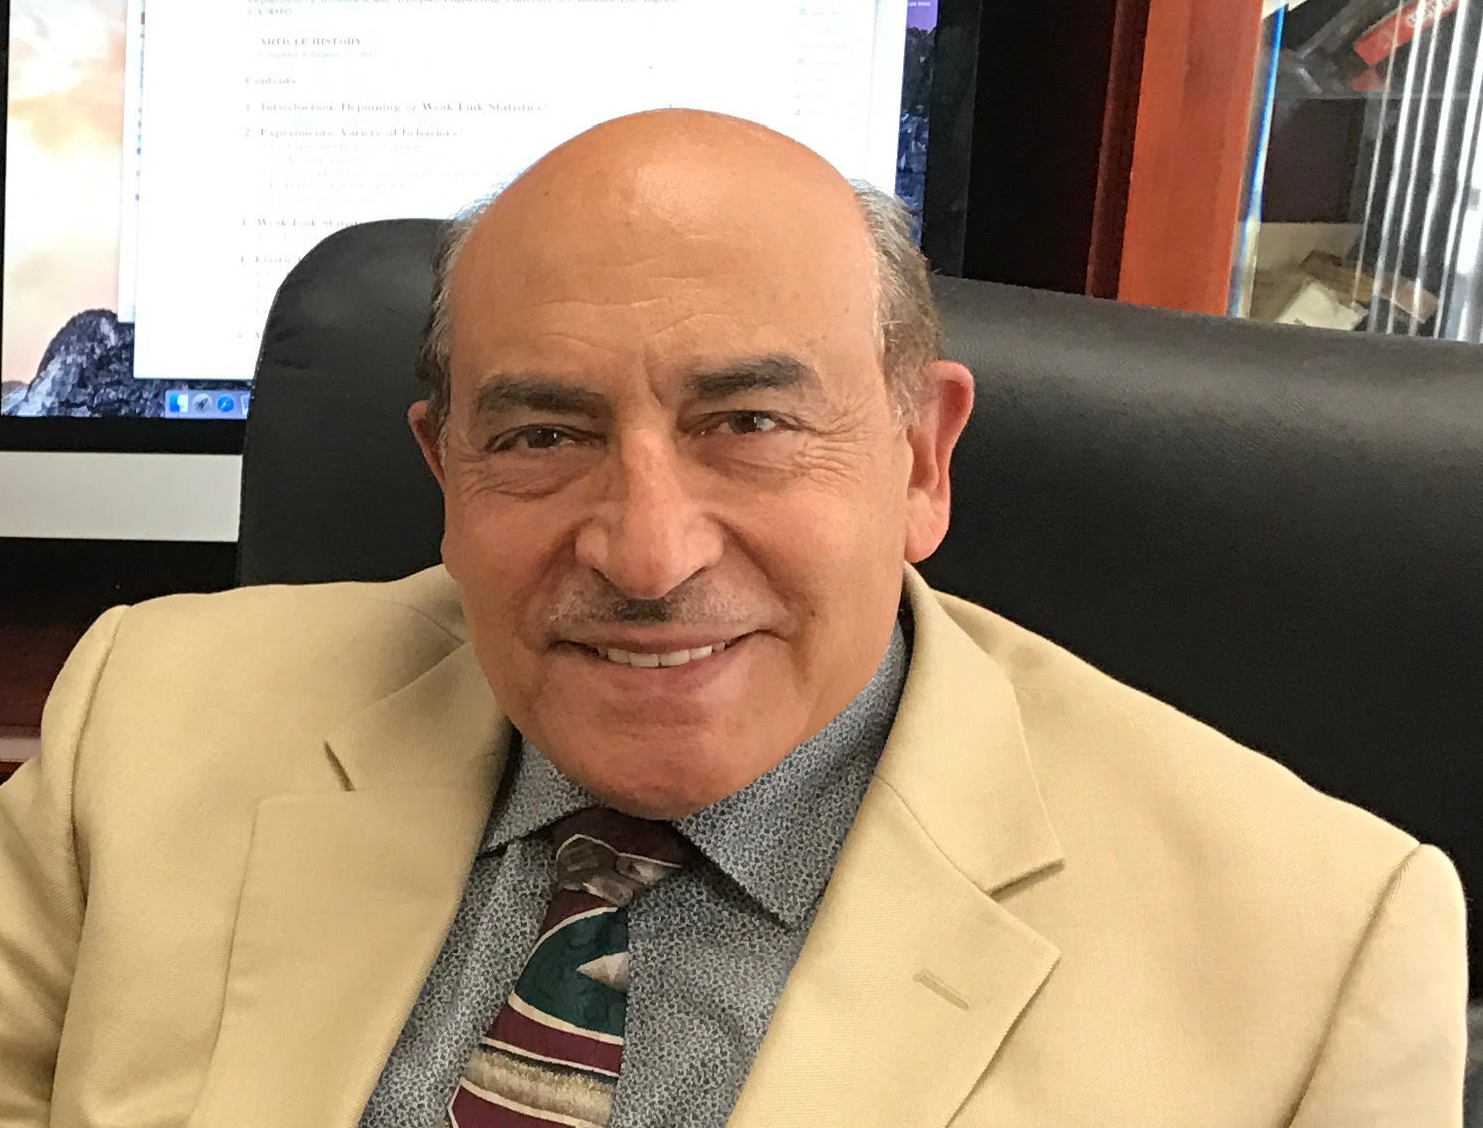
\includegraphics[width=0.4\textwidth]{Nasr-Pic}
\end{wrapfigure}

He was the general chair of the Second International Multiscale Materials Modeling Conference in 2004 and the chair of the 19$^{th}$ International Conference on Fusion Reactor Materials in 2019.  He serves on the editorial boards of several journals and has published over 350 articles, 10 edited books, and is the coauthor of a two-volume book (Oxford Press) on the mechanics and physics of defects, computational materials science, radiation interaction with materials, instabilities, and self-organization in non-equilibrium materials (Oxford Press, 2007, 1100 pages).  He supervised the graduation of 43 Ph.D. students and 25 postdoctoral scholars. 16 of his former students and postdocs are currently professors in various universities around the world, and many of his former students are technology leaders in the United States. 
\section{Course Overview and Objectives}
The Renewable Energy course provides introductory-level tutorials on
conversion principles and technologies in various clean energy sources, such as solar, wind, hydro, biomass, and geothermal. We examine the issues involved in the thermodynamics, design, and operation of three main systems: solar, biomass, and hydropower during the first six weeks of the class. We also discuss the integration of various clean energy sources and their economics. At the completion of this course you will be able to:
\begin{itemize}
    \item Understand the principles of operation of several clean energy technologies.
    \item Analyze the "system" aspects of clean energy technologies.
     \item Realize the technical and economic challenges of each system.
    \item Learn the fundamental principles of thermodynamic energy conversion.
   \end{itemize}


Students are expected to spend 90 minutes per week with the instructor and an additional 1-2 hours per week on homework assignments.
\section{Required Textbook}
\begin{enumerate}
\item Peake, Stephen. \emph{Renewable Energy: Power for a Sustainable Future}, Fourth Edition, 2018, {\bf{Oxford University Press}}, EISBN 978-0-19-253777-5. 
2012.
\item Online lesson content: All other materials are available online through the Neoscholar course website.
\end{enumerate}
\section{Assignments}
Various assignments will be given to students to enhance their learning experience and understanding.  These include:
\begin{itemize}

\item \textbf{Homework Assignments}: Homework assignments
will cover material from multiple lessons per assignment.
\item \textbf{Midterm}: An open-book midterm exam will be held midway through the course.
\item \textbf{Final Assignment}: A literature review assignment on a list of topics provided by the professor will be given on the last day of class.  Students will be required to submit a 500-word abstract summarizing the assigned topic. All assignments will be graded by the teaching assistant.
\end{itemize}
\newpage

\section{Grading}
	
	\begin{table}[h!]
	    \centering
	    \begin{tabular}{|l|l|}
	         	\hline\hline
	Grade Category	& Percent of the Grade		\\
		\hline\hline  
		Homework	& 30\%	\\
		Midterm & 20\%\\
		Final Research Abstract Assignment	& 50\%	\\
		\hline\hline
	    \end{tabular}
	    \caption{Grading Scheme}
	    \label{tab:grades1}
	\end{table}
	
	\begin{table}[h!]
	    \centering
	    \begin{tabular}{|l|l|}
	         	\hline\hline
	Letter Grade	& Percentage		\\
		\hline\hline  
		A+	& $>$95\%	\\
		A	& 90-95\%	\\
		A-	& 85-90\%	\\
		B+	& 80-85\%	\\
		B & 75-80\%\\
		B-& 70-75\%\\
		C&$<70\%$\\
		\hline\hline
	    \end{tabular}
	    \caption{Letter grade percentages}
	    \label{tab:grades2}
	\end{table}
	
	\newpage
	\section{Course Schedule}
	\subsection*{Week 1}
	\begin{itemize}
	    \item Class orientation.
	    \item Global energy use.
	    \item Fossil fuels and climate change.
	    \item Overview of renewable energy sources.
	    \item Reading Assignment: Chapter 1 - Introducing Renewable Energy.
	\end{itemize}
        \subsection*{Week 2}
	\begin{itemize}
\item Energy forms and energy conservation principles.
\item Basic units and definitions.
\item Work and examples of work.
\item Potential and kinetic energy.
\item First law of thermodynamics.
\item Examples of the first law.
        \end{itemize}
	\subsection*{Week 3}
	\begin{itemize}
	   \item Second law of thermodynamics.
	   \item Fuels \& combustion.
	   \item Heat engines.
            \item Heat pumps.
            \item Efficiency and Coefficient of Performance.
	    \item Reading Assignment: Chapter 2 - Thermodynamics, heat engines, and heat pumps.
	\end{itemize}
\subsection*{Week 4}
\begin{itemize}
	   \item Thermodynamic cycles for renewable energy.
	   \item Rankine Cycle.
	   \item Organic Rankine Cycle.
	    \item Reading Assignment:  - Thermodynamic cycles for renewable energy.
	\end{itemize}
\subsection*{Week 5}
	   \begin{itemize}
	   \item Thermodynamic cycles for renewable energy.
	   \item Solar Rankine Cycle.
	   \item Geothermal Cycles.
	    \item Reading assignment: thermodynamic cycles for renewable energy.
	\end{itemize}
 
	\subsection*{Week 6}
	\begin{itemize}
            \item Solar Thermal Energy
            \item Availability of solar energy
            \item Low-temperature applications.
            \item Active versus passive heating.
            \item Generation of electricity from solar thermal sources.
            \item Economics \& environmental impact.
            \item Reading Assignment: Chapter 3 - Solar-Thermal Energy.
	    \end{itemize}
	\subsection*{Week 7}
	\begin{itemize}
        \item Solar Photovolatics
        \item Basic physics
        \item Polycrystalline silicon technology 
         \item Reading Assignment: Chapter 4 - Solar Photovoltaics.
	\end{itemize}

\subsection*{Week 8}
	\begin{itemize}
        \item Thin-film photovolatics.
        \item Advanced high-efficiency multi-layered photovoltaics.
	    \item PV grid-connected systems \& integration.
	    \item Environmental impact \& economics.
	    \item Reading Assignment: Chapter 4 - Solar Photovoltaics.
     \end{itemize}
		\subsection*{Week 9}
	\begin{itemize}
	  \item Bioenergy sources
	    \item Combustion of solid biomass.
	    \item Fuel production (gaseous and liquid).
	    \item Environmental impact \& economics.
	    \item Reading Assignment: Chapter 5 - Bioenergy.
	\end{itemize}
	\subsection*{Week 10}
	\begin{itemize}
	  \item History of water power.
	    \item Hydro resources.
	    \item Types of hydroelectric plants.
	    \item Turbines.
	    \item Integration 
	    \item Environmental impact \& economics.
	    \item Reading Assignment: Chapter 6- Hydroelectricity.
	    % \item Project orientation and team assignments.
	\end{itemize}
	
  
% \newpage
% \section{Project Description}

% Renewable energy sources are important in two respects: (1) they can be sustainable for long periods, and (2) they are carbon-free or have low-carbon emissions.  Nevertheless, many technologies are still emerging and are in the process of intense development. There are many constraints that affect the rapid development and introduction of renewable energy sources. These are mainly economic, but some limitations are also related to society and its acceptance of such technologies. The world will need many
% professionals with a deep knowledge of renewable energy technologies.  Key to such expertise is understanding the 
% underlying physical and technological principles, their economics and market needs, their environmental impact, and the likelihood that they can be integrated within existing energy grids, especially within the concept of "smart grids."

% In this project, a team of students will develop a concept report that addresses one particular renewable energy source, and make a presentation of their findings at the end of the course.  The guidelines for the project, associated report, and group presentation are:
% \begin{enumerate}
%     \item Select a renewable energy source and develop a research plan.  The energy source may be from the following list.
%     \begin{itemize}
%         \item Heat pumps.
%         \item Rooftop solar thermal water heater.
%         \item Domestic solar heating systems.
%         \item Active solar heating and design of solar collectors.
%         \item Passive solar heating of residential and commercial buildings. 
%         \item Solar thermal engines, power plants, and electricity generation.
%         \item Solar photovoltaics: physics \& technology.
%         \item Large, grid-connected Solar photovoltaic power plants.
%         \item Biomass resources.
%         \item Bioenergy conversion technologies.
%         \item Hydroelectric power plants.
%         \item Tidal energy technologies: barrages, lagoons, \& streams.
%         \item Electric power from wind energy.
%         \item Wave energy technology.
%         \item Deep geothermal energy.
%     \end{itemize}
%     \item Make an outline for your project and final report.  Your outline may include some of the following:
%     \begin{itemize}
%         \item Introduction
%         \item History
%         \item Physics \& technology principles
%         \item Description of a typical system, engine, or power plant.
%         \item Integration in the energy grid.
%         \item Environmental impact
%         \item Economics
%         \item Future developments
%         \item Conclusions
%         \item References
%         \item Appendices
%     \end{itemize}
%     \item Perform research on the topic in consultation with the Teaching Assistant and your team members.
%     \item Divide up the report writing tasks amongst team members.
%     \item Prepare the project report as a collaborative effort with the participation of all team members. The report is expected to be between 15-20 pages long.
%     \item Prepare a PowerPoint presentation to the class, to be given on the last day of instruction.
% \end{enumerate}
\end{document}
